\chapter{研究方法}
\label{cha:methodology}

本論文中,我們仍保持 Joris Dormans~\cite{dormans2010adventures} 與 Antonios Liapis~\cite{liapis2013generating} 為求遊戲設計過程抽象化與高階化的訴求。將「Mission/Space 框架」與「Multi-segment 演化」兩種關卡生成方法結合並予以改良,保留了前者追求的遊戲進程之順序性,後者帶來穩定且多樣化的遊戲內容,希冀藉此提升整體遊戲體驗、相輔相成。

圖~\ref{fig:system-framework} 為系統的整體流程圖。遊戲設計師能夠透過巨觀的觀點來構築遊戲體驗流,將遊玩特徵拆分成多項規則,利用生成語法及改寫系統生成出任務圖。依照任務圖中對應的終端節點 (terminal nodes) 轉換為事先建構完成的房型空間,並得到尚未包含遊戲物件的遊戲地圖。接下來,針對動作冒險遊戲我們提出了數項評估遊戲性的適應性函數,採用基因演算法的過程,令各房間遵守適應性函數的限制得到符合訴求的最適解。

\begin{figure}[h]
  \begin{center}
    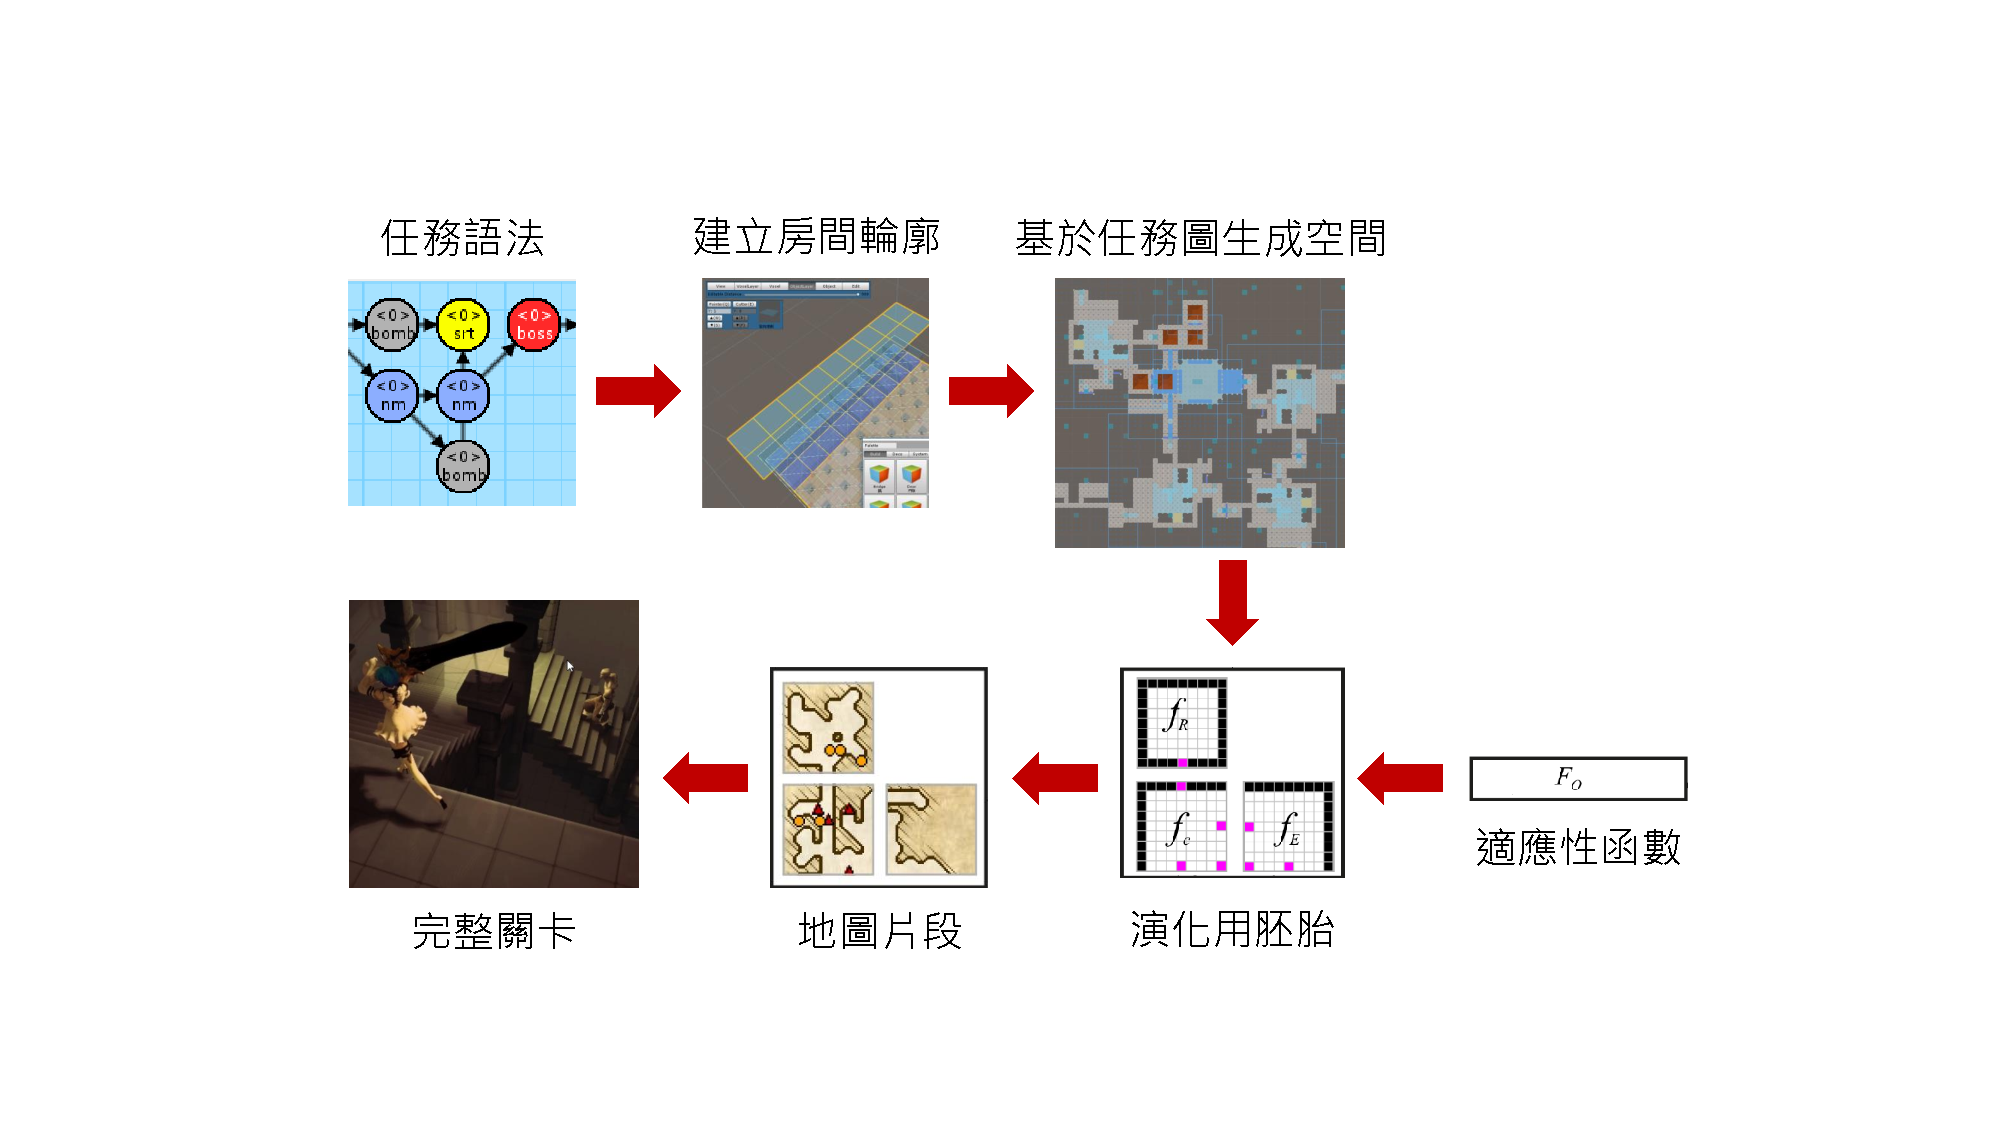
\includegraphics[width=1.0\textwidth]{figures/系統框架.pdf}
    \caption{本論文提出系統之流程圖。} 
    \label{fig:system-framework}
  \end{center}
\end{figure}

關卡產生的遞迴過程如


\section{關卡佈局}
\label{sec:method-levellayout}

關卡佈局,

\section{任務語法}

\label{sec:method-missiongrammars}

我們基於 Joris Dormans 提出之 Mission Grammars 概念,進行實作與改良出 Dungeon Generator 工具,這項工具佈署在 Unity Engine 上。

在任務語法的設計階段,我們參考遊戲 Spiral Knight 的關卡地圖,分析其遊戲進程結構,繪製期望的任務圖並將觀察到的遊玩特徵,接著拆分成任務語法規則使用改寫規則產生出近似結構的任務圖。

\subsection{建立任務字符表}
\label{method-missiongrammars-alphabet}



\subsection{建立任務規則}
\label{method-missiongrammars-rules}


\subsubsection{排除非法規則}
\label{method-missiongrammars-rules-illegals}

設計規則時,Dungeon Generator 將排除不合法的九項設計原則,非法的設計特徵會導致改寫系統出現錯誤,例如:改寫系統陷入無限循環或任務圖破碎化。以下所列舉之條件,彼此有涵蓋部分交集處,因........。

\begin{table}[h]
  \centering
  \caption{非法的任務規則定義}
  \label{tbl:illegal-mission-rules}
  \bigskip
  \begin{tabular}{| p{4cm} | p{9cm} |}
    \hline
    \multicolumn{1}{ |c| }{非法規則之標籤} & \multicolumn{1}{ |c| }{標籤的狀況描述} \\\hline
    LeftMoreThanRight  & 當左側的節點超過右側的節點數量時,進行改寫系統會使左側無法對應到右側的節點產生遺失的情形。若這些節點原先已有與其它非規則內節點連接,將會導致該連接資訊遺失,有機會造成任務圖破碎。 \\\hline
    EmptyLeft          & 左側為空將無法進行子圖搜索,因此左側節點必須至少一個節點。 \\\hline
    IsolatedNode       & 孤立的節點將會導致任務圖破碎。 \\\hline
    IsolatedConnection & 孤立的連接線無法正確表示其連接資訊,將無法正常進行改寫系統。 \\\hline
    ExactlyDuplicated  & 若左右規則同構將導致改寫系統陷入無限循環。 \\\hline
    MultipleRelations  & 兩兩節點間不可有超過一個的連接關係,不論是同向連接線或反向連接線皆會導致改寫系統無法正常運作。 \\\hline
    CyclicLink         & 任務圖的定義中,任務應嚴格遵守任務間之順序性,若有循環結構將會使玩家迂迴停滯。 \\\hline
    OrphanNode         & 若有圖形語法含有兩個以上的根結點,便無法正確定位出任務起點。 \\\hline
    OverflowedAnyNode  & 當右側規則使用 Any 節點時,其對應到左側索引值的節點亦必須為 Any 節點。反之,左側規則使用 Any 節點將不在此限。 \\
    \hline
  \end{tabular}
\end{table}


\subsection{產生任務圖}
\label{method-missiongrammars-graph}

\begin{algorithm}
    \caption{任務語法的改寫系統}
    \label{alg:algorithm-missiongrammars-rewritesystem}
    \begin{algorithmic}
        \IF{some condition is true}
            \STATE do some processing
        \ELSIF{some other condition is true}
            \STATE do some different processing
        \ELSE
            \STATE do the default actions
        \ENDIF
    \end{algorithmic}
\end{algorithm}


\section{房型建構}
\label{method-spacepieces}

Joris Dormans 於文獻中提到為二維空間的範例,我們的實驗環境以三維空間為主。在空間語法中將直接構築遊戲的基礎房型,但不設置怪物、寶箱或陷阱足以直接影響遊戲性的遊戲物件,如圖~\ref{fig:gameobject-list}。此外,我們希望空間中的遊戲物件能夠有意義的自動化配置,即在設計空間語法的流程中,忽略絕大部分的遊戲物件配置,直到~\ref{method-segments} 節提出之方法達成。

\begin{figure}[h]
  \begin{center}
    
\includegraphics[width=1.0\textwidth]{figures/under_construction.png}
    \caption{能夠直接影響遊戲性的遊戲物件,分別為敵方、寶箱與陷阱。} 
    \label{fig:gameobject-list}
  \end{center}
\end{figure}

我們對於空間語法做了修改以利實驗環境建置。圖~\ref{fig:spacepieces-structure} 所示,在一個關卡 (level) 中包含數個房間容器 (volumes),每一房間由不定數量的房間塊 (chucks) 組成,且房間塊固定以 9x9x9 個長方體體素 (voxels) 所構成,每一體素的大小為 3x2x3。為了要從已生成完畢的任務圖再衍生出分支的遊戲空間,在創建的房間容器會對應一任務語法之字符表當中一的終端符 (terminal symbols),這樣的關係稱作為建造指示 (building instruction);若在改寫規則運行中,且有多項規則同時符合替換的條件時,系統會基於它們的關聯權重 (relative weight) 隨機挑選一個規則。

\begin{figure}[h]
  \begin{center}
    
\includegraphics[width=1.0\textwidth]{figures/under_construction.png}
    \caption{房型之結構圖。} 
    \label{fig:spacepieces-structure}
  \end{center}
\end{figure}

此外,每一個體素被分為九種方向,分別為正四方、斜四方與中心點。不同的裝飾物會依照其特性決定能夠放置的方位,如牆壁放置於正四方;牆壁柱放置於斜四方;地面或階梯則放置於中心點。在一個體素中,多個裝飾物是能夠同時並存的,例如在其放置地面、一道牆壁、兩道牆壁柱。在本次實驗環境中,我們將會使用「地面、階梯、牆壁、牆壁柱、門」共五種裝飾物進行房型的建置工作。

\begin{figure}[h]
  \begin{center}
    
\includegraphics[width=1.0\textwidth]{figures/under_construction.png}
    \caption{裝飾物放置於體素結構的情形示意。} 
    \label{fig:decorations-with-directions}
  \end{center}
\end{figure}

\section{地圖片段}
\label{method-segments}

延續上一小節的關卡結構,房間視為單一染色體 (chromosome) 之個體 (individual);房間中能夠放置遊戲物件的各點座標視為基因 (genes),而基因的類型有空磚、怪物磚、寶箱磚與陷阱磚等;同一個房間會擁有多種不同遊戲物件配置情況的染色體,這些染色體的集合便是族群 (population)。第一步驟,產生初始父母代族群時,讓全部的基因先預設為空磚,並使各染色體先行隨機突變;第二步驟,透過適應性函數計算各染色體的適應值 (fitnesses),完整的適應性函數在~\ref{method-segments-fitnesses} 小節中說明;第三步驟將會從族群中挑選最優異的兩個父母染色體,高機率進行交配,若無進行交配將會將子代沿用父母代的基因,採用的交配方法在~\ref{method-segments-crossover} 小節中說明;第四步驟有低機率讓衍生的子代進行突變,不同的突變方式於~\ref{method-segments-mutation} 小節中說明;第五步驟以新的衍生子代取代舊有的父母代族群;第六步驟會檢查是否達到終止條件,若尚未滿足終止條件,便會回到第二步驟,直到輸出最佳解。

\subsection{演化之適應性函數}
\label{method-segments-fitnesses}

動作冒險遊戲 (A-AVG)、動作角色扮演遊戲 (A-RPG) 等類型遊戲,多可見一些制式化遊戲物件的搭配組合,我們嘗試汲取出多項遊玩特徵並參數化公式,作為評估關卡品質的指標之一。在前處理時,我們使用 A-Star 演算法尋找入口至多個出口的最短路徑,凡經過的座標稱作為空間動線 ($MP$) 之一,並將其權重值 ($mp$) 增加一,空間動線為多項指標關鍵性的參考依據。

\subsubsection{守衛點 (Guard)}
\label{method-segments-fitnesses-guard}

為體現出敵人會保衛寶箱 ($T$) 與出口 ($E$) 的現象,計算敵人 ($E_{i}$) 與關鍵性較高遊戲物件 ($O_{j}$) 之間的距離,倘若距離愈近則帶來的影響力愈大。

\begin{equation}
    f_{grd}=\frac{1}{N \times M} \sum_{i=1}^{N} \sum_{j=1}^{M} \frac{1}{dist\big(E_{i}, O_{j}\big)}, O_{j} \in \{ Treasure, Exit \}
\end{equation}

\subsubsection{阻攔點 (Block)}
\label{method-segments-fitnesses-block}

敵人會專注於阻擋玩家繼續前進,迫使玩家與其發生衝突。敵人會配置於動線上,$mp_{i}$ 為空間動線權重;$e_j$ 為該敵人於空間之動線權重,倘敵人並未落在動線上,則該項為 0。

\begin{equation}
    f_{blk}=\log _{\sum_{i=1}^{N} mp_{i}} \sum_{j=1}^{M} e_{j}
\end{equation}

\subsubsection{攔截點 (Intercept)}
\label{method-segments-fitnesses-intercept}

與阻攔點近似,但敵人會被配置於動線附近非動線上,以快速追擊玩家為目的。各敵人 ($E_{i}$) 越接近空間動線各點 ($MP_{j}$) 時影響愈大,且動線權重 ($mp_{j}$) 亦會影響加權程度。

\begin{equation}
    f_{itc} = \frac{1}{N \times M} \sum_{i=1}^{N} \sum_{j=1}^{M} \Big( \frac{1}{dist(E_{i}, MP_{j})} \times mp_{j} \Big), 
    E_{i} \neq MP_{j}
\end{equation}

\subsubsection{巡邏點 (Patrol)}
\label{method-segments-fitnesses-patrol}

確保各敵人擁有足夠的空間能夠進行移動。將計算敵人 ($E_{i}$) 與指定半徑 ($r$) 內的座標數量 ($P_j$) 總值,當中並不包含不可通行的牆壁等類型。於本次實驗中,我們將採用 $R=3$ 作為實驗範例,該數值可由遊戲設計師決定。

\begin{equation}
    % The old one: f_{ptl}=\sum_{i=1}^{N} \sum_{j=1}^{M} count\big(E_{i}, P_{j}\big), dist\big(E_{i}, P_{j}\big) \leq r, P_{j} \notin \{ wall \}
    f_{ptl} = \sum_{i=1}^{N} \Big( d_{i} \times \sum_{j=1}^{M} count\big(E_{i}, P_{j}\big) \Big), 
    d_{i} = \begin{cases}
                \frac{1}{2^{i}},   & \mbox{if } i \neq N \\
                \frac{1}{2^{i-1}}, & \mbox{if } i = N
            \end{cases}
\end{equation}
\begin{gather*}
    dist\big(E_{i}, P_{j}\big) \leq r,  P_{j} \notin wall
\end{gather*}

\subsubsection{至高點 (Dominated)}
\label{method-segments-fitnesses-dominated}

當玩家可能所在動線上之位置 ($MP_{j}$) 與敵人的位置 ($E_{i}$) 具有高低差時,敵人便適合採取遠程攻擊;為了提供玩家思考對付遠程敵人的緩衝時間,將敵人配置於動線末端附近是較好的選擇,$j$ 隨著動線的順序演進,影響程度逐漸增幅。

\begin{equation}
f_{dom}=\sum_{i=1}^{N} \sum_{j=1}^{M} \Big( \frac{1}{dist\big(E_{i}, MP_{j}\big)} \times mp_{j} \times j \times high(E_{i}, MP_{j}) \Big)
\end{equation}

\subsubsection{支援點 (Support)}
\label{method-segments-fitnesses-support}

敵人 ($E_{i}$, $E_{j}$) 之間擁有一定程度的護援關係,當敵人彼此的距離愈低其影響程度越大,同時該敵人 ($E_{i}$) 必須遠離動線 ($MP_{k}$)。

\begin{equation}
f_{sup}=\frac{1}{N} \sum_{i=1}^{N} \bigg( \frac{1}{N} \sum_{\substack{j=1 \\ j \neq i}}^{N} \frac{1}{dist(E_{i}, E_{j})} + \frac{1}{M} \sum_{k=1}^{M} \frac{1}{dist(E_{i}, MP_{k})} \bigg)
\end{equation}

\subsubsection{死角點 (Neglected)}
\label{method-segments-fitnesses-neglected}

由於房與房之間的牆壁阻隔,使得敵人能夠埋伏於入口附近之死角處,出奇不意地對玩家展開攻擊。為了體現出這種現象,我們將敵人 ($E_{i}$) 與主要動線上各點 ($MP_{i}$),兩端點連線之對角線所構成的立方體,立方體所涵蓋各座標點 ($N_{j}$) 至該對角線的距離為 $d_{k}$,隨著距離增加影響程度會衰減;$vis_{k}$ 為該點的可視情形,若有不可視的座標存在便會提高適應值。隨著動線的順序演進,影響程度逐漸衰減。

\begin{equation}
Under construction
\end{equation}

% \subsubsection{點 ()}
% \label{method-segments-fitnesses-}

% \subsubsection{點 ()}
% \label{method-segments-fitnesses-}

\subsection{負數權重的適應性函數}
\label{method-segments-minusscores}

在~\ref{method-segments-fitnesses-guard} 守衛點指標的設計中,當權重為正數時能夠體現出「需要被守護的物件周圍出現敵方單位進行守衛」的遊玩特徵,且在多個物件的情形下儘可能平均分配敵方單位;反之,負數權重便會體現出「愈不平均數量的守衛情形」。緣故為設計守衛點指標時,並無針對寶箱的數量進行控管而導致。

\subsection{多項適應性函數合併}
\label{method-segments-multiobjectives}

在設計適應性函數初期,為求多個適應性函數相互牽制,進而求得限制條件的最佳解。而初期函數會力求場上所有的敵人必須盡可能符合各項指標,舉例來說,在某一房型的設定中,我們將守衛點、阻攔點的權重調整至 1,其餘指標將不採計得分即不調整權重,倘若場面上存在著二個敵人 A 與 敵人 B,他們會同時被設置在動線上且一定距離內會有作為守護對象的寶箱物件。但對於遊戲設計師在某些情形下,敵人 A 與敵人 B 僅需要分別符合守衛點、阻攔點指標,才是理想中的遊玩特徵。因此,我們定義首次出現相關遊玩特徵的得分將會最高,並依照數量逐漸下降成長幅度且逼近於 1,呈現近似於底數大於 1 的對數函數圖形。藉著取代原先的線性成長關係以外,便可以達到數值的正規化,強制將值域上限規範至 1 以求最後適應性函數加權總分時,不偏袒任何適應性函數以達到公平基準。

然而在對數函數中,當真數為 1(符合指標的敵人數量為 1)時,所得之值為 0 並不符合我們的訴求。

\subsection{不同交配方式}
\label{method-segments-crossover}



\subsection{不同的突變方式}
\label{method-segments-mutation}



\subsection{終止條件的設立}
\label{method-segments-termination}


